\documentclass[paper=a4, fontsize=11pt]{scrartcl} % KOMA-article class

%-------------------------------------------------
%   THEMES, PACKAGES, CUSTOM COMMANDS
%-------------------------------------------------
\usepackage{blindtext}
\usepackage[english]{babel}                             % English language/hyphenation
\usepackage[protrusion=true,expansion=true]{microtype}  % Better typography
\usepackage{amsmath,amsfonts,amsthm}                    % Math packages
\usepackage[pdftex]{graphicx}                           % Enable pdflatex
\usepackage[export]{adjustbox}
\usepackage[svgnames]{xcolor}                           % Enabling colors by their 'svgnames'
\usepackage[hang, small,labelfont=bf,up,textfont=it,up]{caption} % Custom captions under/above floats
\usepackage{subcaption}
\usepackage{caption}
\usepackage{epstopdf}       % Converts .eps to .pdf
%\usepackage{subfig}         % Subfigures
\usepackage{booktabs}       % Nicer tables
\usepackage{fix-cm}         % Custom fontsizes
\usepackage{listings}
\usepackage{soul}
\usepackage{float}

\usepackage{hyperref}

\usepackage[foot=30pt,margin=1in]{geometry}

\usepackage{listings}
\definecolor{mygreen}{rgb}{0,0.6,0}
\definecolor{mygray}{rgb}{0.5,0.5,0.5}
\definecolor{mymauve}{rgb}{0.58,0,0.82}
\lstset{ %
    backgroundcolor=\color{white},   % choose the background color; you must add \usepackage{color} or \usepackage{xcolor}
    basicstyle=\footnotesize,        % the size of the fonts that are used for the code
    breakatwhitespace=false,         % sets if automatic breaks should only happen at whitespace
    breaklines=true,                 % sets automatic line breaking
    captionpos=b,                    % sets the caption-position to bottom
    commentstyle=\color{mygreen},    % comment style
    deletekeywords={...},            % if you want to delete keywords from the given language
    escapeinside={\%*}{*)},          % if you want to add LaTeX within your code
    extendedchars=true,              % lets you use non-ASCII characters; for 8-bits encodings only, does not work with UTF-8
    frame=single,                    % adds a frame around the code
    keepspaces=true,                 % keeps spaces in text, useful for keeping indentation of code (possibly needs columns=flexible)
    keywordstyle=\color{blue},       % keyword style
    language=Python,                 % the language of the code
    morekeywords={*,...},            % if you want to add more keywords to the set
    numbers=left,                    % where to put the line-numbers; possible values are (none, left, right)
    numbersep=5pt,                   % how far the line-numbers are from the code
    numberstyle=\tiny\color{mygray}, % the style that is used for the line-numbers
    rulecolor=\color{black},         % if not set, the frame-color may be changed on line-breaks within not-black text (e.g. comments (green here))
    showspaces=false,                % show spaces everywhere adding particular underscores; it overrides 'showstringspaces'
    showstringspaces=false,          % underline spaces within strings only
    showtabs=false,                  % show tabs within strings adding particular underscores
    stepnumber=2,                    % the step between two line-numbers. If it's 1, each line will be numbered
    stringstyle=\color{mymauve},     % string literal style
    tabsize=3,                       % sets default tabsize to 2 spaces
    title=\lstname                   % show the filename of files included with \lstinputlisting; also try caption instead of title
}

% Custom sectioning (sectsty package)
\usepackage{sectsty}
\allsectionsfont{
    \usefont{OT1}{phv}{b}{n}    % bch-b-n: CharterBT-Bold font
}
\sectionfont{
    \usefont{OT1}{phv}{b}{n}
}

% Custom colors
\definecolor{brsugrey}{rgb}{0.9, 0.9, 0.9}
\definecolor{brsublue}{rgb}{0, 0.594, 0.949}

%
\newcommand{\upperRomannumeral}[1]{\uppercase\expandafter{\romannumeral#1}}

% Creating an initial of the very first character of the content
\usepackage{lettrine}
\newcommand{\initial}[1]{%
    \lettrine[lines=3,lhang=0.3,nindent=0em]{
        \color{brsublue}
        {\textsf{#1}}}{}}

%-------------------------------------------------
%   COMMON INFO
%-------------------------------------------------
\newcommand{\hmwkTitle}{MNIST Digit Classification Report}
\newcommand{\hmwkDueDate}{Monday, December 11, 2016}
\newcommand{\hmwkClass}{Scientific Evaluation and Experimentation}
\newcommand{\hmwkClassShort}{SEE WS2016}
\newcommand{\hmwkAuthorFullName}{Minh H. Nguyen \& Bach D. Ha}
\newcommand{\hmwkAuthorLastName}{Nguyen \& Ha}
\newcommand{\hmwkAuthorEmail}{minh.nguyen@smail.inf.h-brs.de\\
                              bach.ha@smail.inf.h-brs.de}
\newcommand{\hmwkAuthorInstitute}{BRS University of Applied Sciences}

%-------------------------------------------------
%   HEADERS & FOOTERS
%-------------------------------------------------
\usepackage{fancyhdr}
\pagestyle{fancy}
\usepackage{lastpage}
% Header (empty)
\lhead{}
\chead{}
\rhead{}
% Footer (you may change this to your own needs)
\lfoot{\footnotesize
    \texttt{\hmwkClassShort} ~
    \textbullet ~ \hmwkAuthorLastName ~
    \textbullet ~ \hmwkTitle}
\cfoot{}
\rfoot{\footnotesize page \thepage\ of \pageref{LastPage}}  % "Page 1 of 2"
\renewcommand{\headrulewidth}{0.0pt}
\renewcommand{\footrulewidth}{0.4pt}

%-------------------------------------------------
%   TITLE & AUTHOR
%-------------------------------------------------
\usepackage{titling}

\newcommand{\HorRule}{\color{brsublue}% Creating a horizontal rule
    \rule{\linewidth}{1pt}%
    \color{black}
}

% Title
\pretitle{
    \vspace{-30pt}
    \begin{flushleft}
        \HorRule
        \fontsize{22}{22} \usefont{OT1}{phv}{b}{n} \color{gray} \selectfont
}
\title{\hmwkClass \\
       \hmwkTitle}
\posttitle{
    \par
    \end{flushleft}
    \vskip 0.5em
}

% Author
\preauthor{
    \begin{flushleft}
        \large \lineskip 0.25em
        \usefont{OT1}{phv}{b}{sl} \color{brsublue}}

\author{\hmwkAuthorFullName}

\postauthor{
        \footnotesize
        \usefont{OT1}{phv}{m}{sl} \color{Black}
        \\\hmwkAuthorInstitute
        \\\hmwkAuthorEmail
        \par
    \end{flushleft}
    \HorRule}

% Date
\date{\hmwkDueDate}

%-------------------------------------------------
%   BEGIN
%-------------------------------------------------
\begin{document}
    \maketitle
    \thispagestyle{fancy} % Enabling the custom headers/footers for the first page

\section{Digit Classification using Convolutional Neural Networks (CNN)}
    \subsection*{Model}
    Use a CNN model with for digit classification. The model is created using Python deep learning library Keras. The model is visualized in figure \ref{fig:model}.
    \begin{figure}[H]
        \begin{center}
            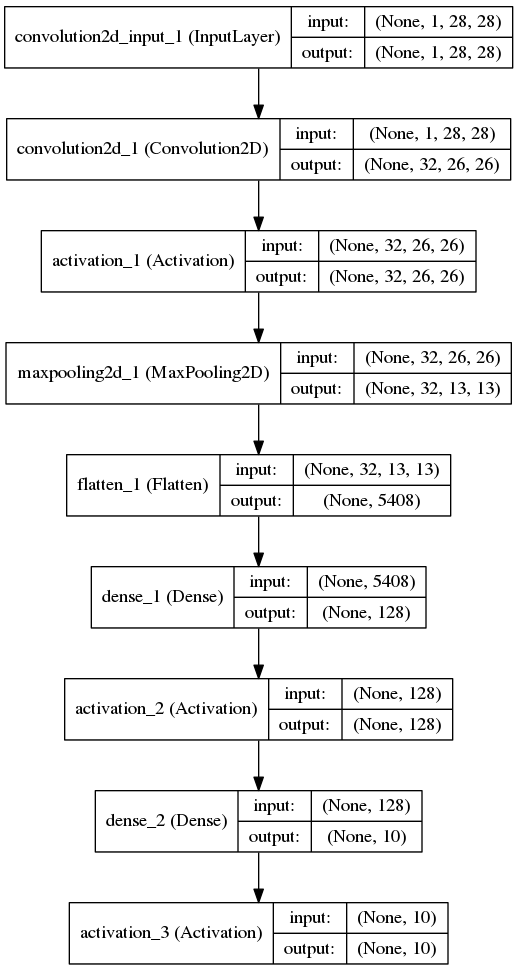
\includegraphics[width=0.6\linewidth]{images/mnist_model.png}
            \caption{Convolution model}
            \label{fig:model}
        \end{center}
    \end{figure}

    \subsection*{Training}
    The model is optimized using a categorical cross entropy loss function with ada delta method. The network is run for 150 epochs. The weights are visualized in figure \ref{fig:weights}, and accuracy for each epoch are plotted in figure \ref{fig:train}.
    \begin{figure}[H]
        \begin{center}
            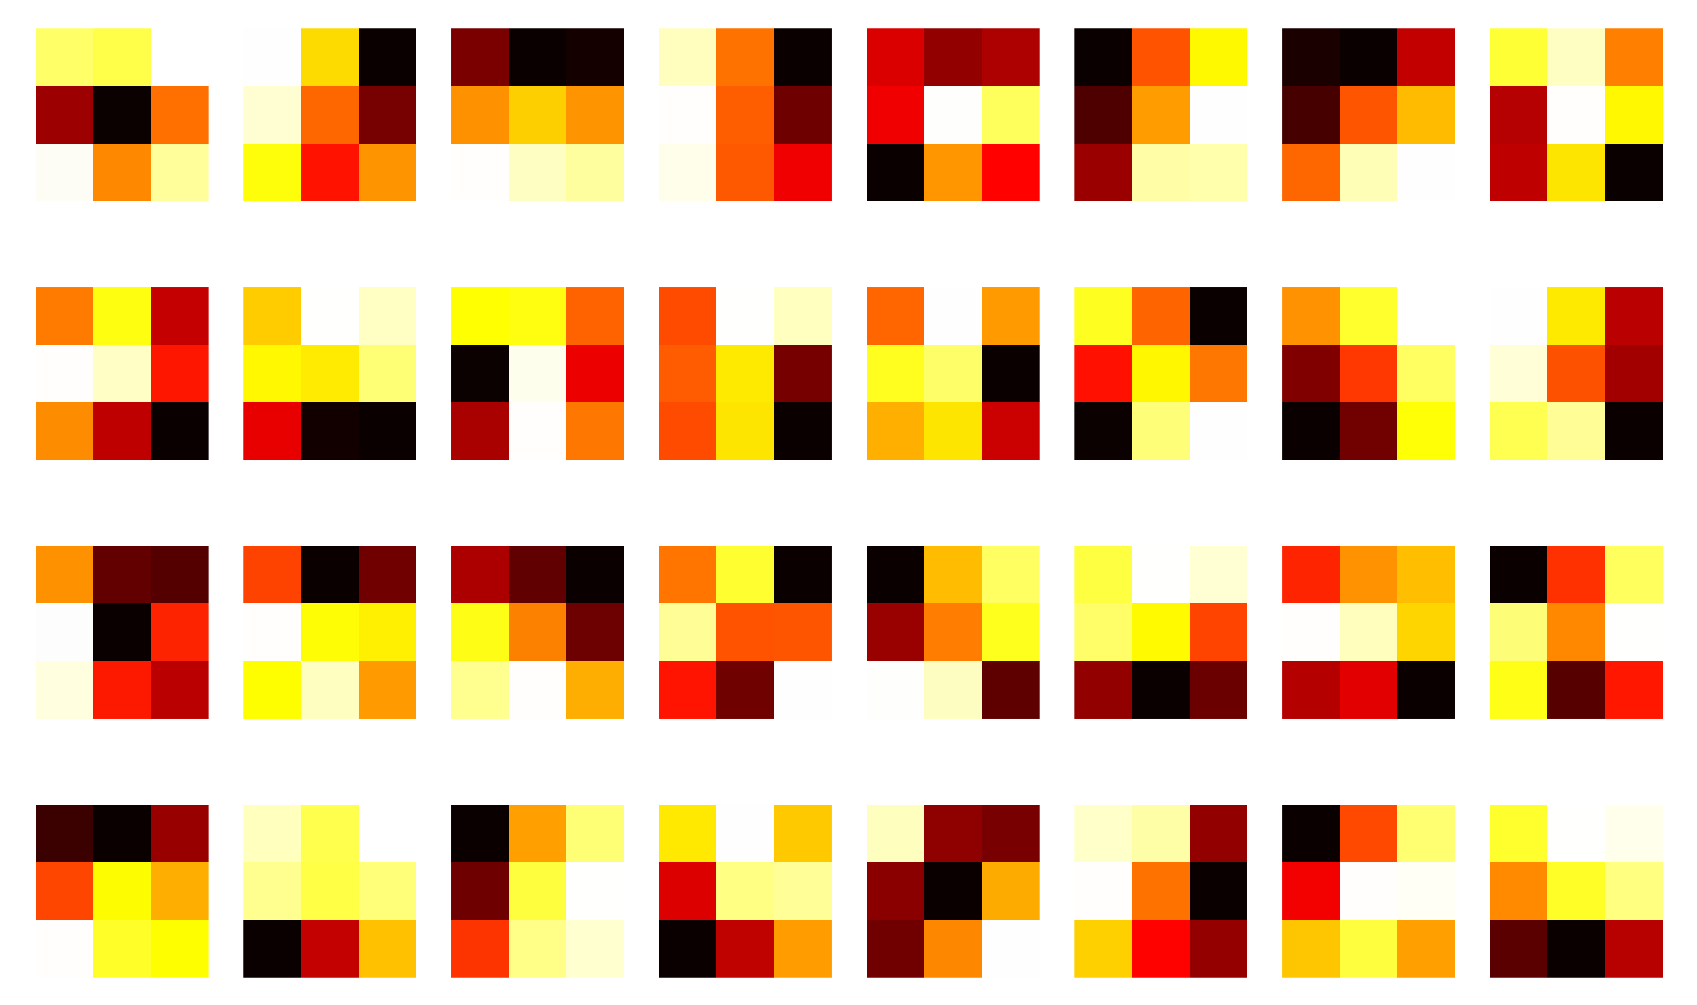
\includegraphics[width=1.0\linewidth]{images/mnist_weights.png}
            \caption{Model weights visualization}
            \label{fig:weights}
        \end{center}
    \end{figure}
	Looking at the weights visualization, it can be seen that some of them resemble kernels, which are used in computer vision. In this case edge detecting kernels are the easiest to see.

    \begin{figure}[H]
        \begin{center}
            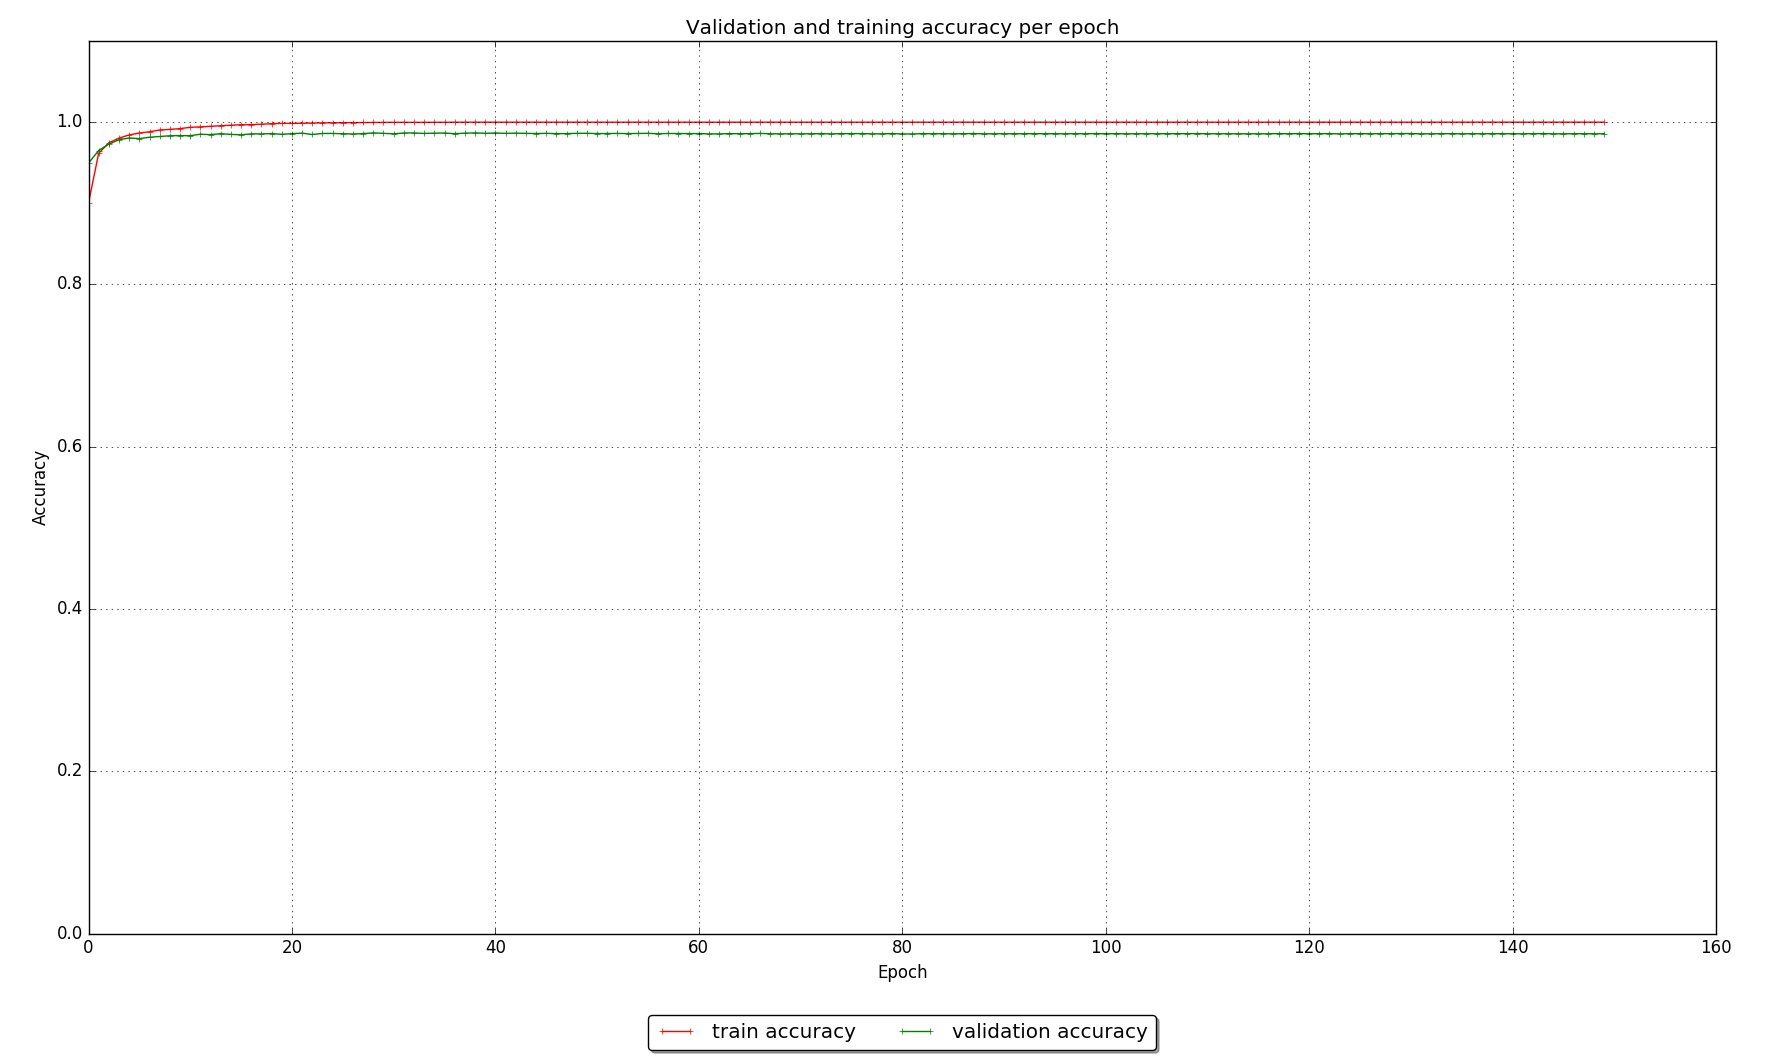
\includegraphics[width=1.0\linewidth]{images/mnist_training_log.png}
            \caption{Accuracy per epoch}
            \label{fig:train}
        \end{center}
    \end{figure}
	
	\begin{itemize}
		\item With the split ratio of 0.33 for the test set, the performance is good.
		\item After the first epoch, the accuracy reaches over 0.95.
		\item The network converge somewhere around epoch number 25 with the accuracy of 0.986
		\item There seems to be no overfitting at all, even after 150 epochs.
	\end{itemize}
	

\section{Results}
    Test score: $0.0852$ \\
    Test accuracy: $0.986$ \\
    Confusion matrix: \\
    The row represents the true value, the column represents the predicted value.\\
    From the top left corner, each rows and column represent the label from 0 to 9.
    \[ \left[ \begin{array}{cccccccccc}
        2236 &    0 &    4 &    0 &    1 &    3 &    2 &    2 &    5 &    3 \\
           0 & 2553 &    7 &    1 &    2 &    1 &    0 &    4 &    2 &    1 \\
           4 &    3 & 2239 &    6 &    6 &    0 &    1 &   17 &    5 &    2 \\
           3 &    1 &    6 & 2398 &    0 &   29 &    0 &    4 &    9 &    4 \\
           3 &    3 &    1 &    0 & 2207 &    0 &    3 &    5 &    1 &   11 \\
           3 &    0 &    1 &    8 &    3 & 2092 &    5 &    0 &    9 &    5 \\
           6 &    5 &    0 &    0 &    3 &    7 & 2229 &    0 &    4 &    0 \\
           1 &    3 &    6 &    2 &    3 &    2 &    0 & 2391 &    1 &    5 \\
           3 &    4 &    5 &    6 &    4 &    9 &    3 &    1 & 2213 &    7 \\
           3 &    1 &    0 &    3 &   14 &    1 &    0 &   10 &   11 & 2210 \\
    \end{array} \right] \]
    
    \begin{itemize}
    	\item The most mislabeled case is 3 being label as 5 with 29 misclassification.
    	\item 9 being classified as 4, 2 as 7, 9 as 7, 4 as 9 are also some bad cases.
    	\item The interesting case is that 9 was never classified as 6 and vice-versa, this can be concluded that the classifier only tolerate a small amount of change in orientation.
    \end{itemize}


\section{Code}
\begin{lstlisting}
def categorial_to_number(label):
    shape = np.shape(label)
    v = np.arange(shape[1]).reshape(-1,1)
    return np.dot(label,v)

def test_network(model, X_test, Y_test):
    acc = 0
    wrong_list = list()
    predicts = np.round(model.predict(X_test))
    predicts = categorial_to_number(predicts)
    Y_test = categorial_to_number(Y_test)

    c_matrix = confusion_matrix(Y_test, predicts)
    for n in range(len(X_test)):
        if (np.allclose(predicts[n],Y_test[n])):
            acc = acc + 1.0
            else:
            #Wrong index, predicted label, true label
            wrong_list.append((n, predicts[n][0], Y_test[n][0]))
            pass
        pass

    print(acc/len(X_test))
    return acc, wrong_list, c_matrix


def create_model(nb_classes, batch_size):
    from keras.models import Sequential
    from keras.layers import Dense, Dropout, Activation, Flatten
    from keras.layers import Convolution2D, MaxPooling2D

    # number of convolutional filters to use
    nb_filters = 32
    # size of pooling area for max pooling
    pool_size = (2, 2)
    # convolution kernel size
    kernel_size = (3, 3)

    model = Sequential()
    model.add(Convolution2D(nb_filters, kernel_size[0], kernel_size[1],
    border_mode='valid', input_shape=(1,28,28)))
    model.add(Activation('relu'))
    model.add(MaxPooling2D(pool_size=pool_size))
    model.add(Flatten())
    model.add(Dense(128))
    model.add(Activation('relu'))
    model.add(Dense(nb_classes))
    model.add(Activation('softmax'))
    
    model.compile(loss='categorical_crossentropy', optimizer='adadelta',
    metrics=['accuracy'])
    return model


def main(num_epoch):
    date_string = time.strftime("%Y%m%d")
    np.random.seed(1337)  # for reproducibility
    mnist = fetch_mldata('MNIST original')

    data = mnist.data.reshape((len(mnist.data),1,28,28))
    data = data.astype('float32')
    data = data/255

    testset_ratio = 0.33
    X_train, X_test, Y_train, Y_test = train_test_split(data, mnist.target.astype('int'), test_size=testset_ratio)

    # convert class vectors to binary class matrices
    from keras.utils import np_utils
    nb_classes = 10
    batch_size = 128
    nb_epoch = num_epoch
    Y_train = np_utils.to_categorical(Y_train, nb_classes)
    Y_test = np_utils.to_categorical(Y_test, nb_classes)

    base_name = "mnist_%s" % date_string
    model = create_model(nb_classes, batch_size)
    model_json = model.to_json()
    model_file_name = base_name + "_model.json"
    with open(model_file_name, "w") as json_file:
    json_file.write(model_json)
    pass
    
    from keras.callbacks import CSVLogger
    csv_logger = CSVLogger("%s_training.log" % base_name, append=False)
    
    model.fit(X_train, Y_train, batch_size=batch_size, nb_epoch=nb_epoch,
    verbose=1, validation_data=(X_test, Y_test), callbacks=[csv_logger])
    model.save_weights(base_name + "_weights.h5")
    score = model.evaluate(X_test, Y_test, verbose=0)
    print('Test score:', score[0])
    print('Test accuracy:', score[1])

    acc, w, c_matrix = test_network(model, X_test, Y_test)
    print(c_matrix)
    return

\end{lstlisting}


%\begin{thebibliography}{9}
%    \bibitem{Thrun}
%    S. Thrun et al., “Velocity Motion Model,” in Probabilistic Robotics, ch. 5, pp. 121–132, Cambridge,
%    MA: The MIT Press, 2006.
%\end{thebibliography}
\end{document}
